\documentclass[10pt,journal,compsoc,onecolumn]{IEEEtran}
\usepackage[utf8]{inputenc}
\usepackage{amsmath,amsfonts,amssymb}
\usepackage{amsthm}
\usepackage{graphicx}
\usepackage{cite}
\usepackage{textcomp}
\usepackage{tikz}
\usetikzlibrary{arrows,positioning,shapes.geometric}
\usepackage{booktabs}
\usepackage{url}

\newtheorem{theorem}{Theorem}
\newtheorem{lemma}[theorem]{Lemma}
\newtheorem{definition}[theorem]{Definition}
\newtheorem{corollary}[theorem]{Corollary}

\begin{document}

\title{On the Algorithmic and Mathematical Foundations of Combinatorics and Prime Number Generation: A Formal Analysis of Counting Principles, Permutations, Combinations, and the Sieve of Eratosthenes}

\IEEEtitleabstractindextext{%
\begin{abstract}
This paper presents a formal analysis of basic counting principles, permutations, combinations, and prime number generation. We explore the product rule and sum rule, detailing their applications in food combo planning and network path routing. We formalize permutations and combinations, proving the algebraic relations for Pascal's identity. We then investigate the Sieve of Eratosthenes for prime number generation. We provide a rigorous proof of the $O(N \log \log N)$ asymptotic time complexity bound of the sieve, illustrate its execution up to $N=30$ with custom TikZ-rendered grid visualizations, and detail standard optimizations including odd-only sieving and segmented sieves. Complete Java reference implementations are provided for all core algorithms.
\end{abstract}

\begin{IEEEkeywords}
binary trees, algorithms, data structures, computational complexity, tree traversal, recursive algorithms, formal analysis
\end{IEEEkeywords}
}

\maketitle
\IEEEdisplaynontitleabstractindextext
\IEEEpeerreviewmaketitle

\section{Introduction}
\label{sec:intro}

Combinatorics and number theory form the mathematical foundation of computer science. While combinatorics deals with the structures, arrangements, and configurations of discrete objects, number theory explores the fundamental properties of integers, with a particular focus on prime numbers. These fields are not merely theoretical; they are crucial in algorithm analysis, cryptography, network routing, database query optimization, and resource allocation.

This paper presents a formal analysis of basic counting principles, permutations, combinations, and prime number generation. We explore the following core topics based on fundamental algorithmic lecture notes:
\begin{enumerate}
    \item \textbf{Basic Counting Rules (\S\ref{sec:counting}):} The product (multiplication) and sum (addition) rules, showing their applications in database query planning (e.g., Zomato meal combo options) and network routing (e.g., multi-city transit paths).
    \item \textbf{Permutations and Selections (\S\ref{sec:permutations}):} The mathematical derivation of permutations ($^nP_r$) and combinations ($^nC_r$), proving their relationship and demonstrating Pascal's identity.
    \item \textbf{Primality Generation (\S\ref{sec:primes}):} The generation of all prime numbers up to $N$ using the Sieve of Eratosthenes, illustrated with a custom TikZ-based grid visualization for $N=30$.
    \item \textbf{Asymptotic Analysis (\S\ref{sec:complexity}):} A rigorous proof of the $O(N \log \log N)$ time complexity of the Sieve of Eratosthenes using Mertens' Theorem and the prime reciprocal sum.
\end{enumerate}

Java reference implementations are provided for the primary algorithmic problems to establish a complete implementation model.

\section{Basic Counting Principles}
\label{sec:counting}

We formalize the two basic rules of counting: the product rule and the sum rule. These principles are based on set theory and form the foundation of discrete probability.

\subsection{The Product Rule (Multiplication Principle)}
\begin{definition}[Product Rule]
If a compound decision can be broken down into a sequence of $k$ independent sub-decisions, where the first sub-decision can be made in $n_1$ ways, the second in $n_2$ ways, and the $i$-th in $n_i$ ways, then the entire sequence of decisions can be made in:
\[
N_{\text{product}} = \prod_{i=1}^{k} n_i = n_1 \times n_2 \times \dots \times n_k
\]
ways.
\end{definition}

In terms of set theory, the product rule describes the cardinality of the Cartesian product of $k$ finite sets:
\[
|S_1 \times S_2 \times \dots \times S_k| = |S_1| \times |S_2| \times \dots \times |S_k|
\]

\subsubsection{Application: Zomato Meal Combos}
In modern e-commerce and food delivery services like Zomato, restaurants offer meal combos consisting of one main course, one dessert, and one beverage. Let a restaurant $i$ have:
\begin{itemize}
    \item $M_i = A[i][0]$ main courses,
    \item $D_i = A[i][1]$ desserts,
    \item $B_i = A[i][2]$ beverages.
\end{itemize}
By the product rule, the total number of distinct meal combos that restaurant $i$ can offer is:
\[
C_i = M_i \times D_i \times B_i
\]
Given a matrix $A$ where each row represents a restaurant's offerings, the problem of finding the restaurant with the highest variety of combos reduces to finding:
\[
i^* = \arg\max_{i} \left( A[i][0] \times A[i][1] \times A[i][2] \right)
\]

\subsection{The Sum Rule (Addition Principle)}
\begin{definition}[Sum Rule]
If a decision can be made in one of $k$ mutually exclusive and disjoint ways, where the first way has $m_1$ options, the second has $m_2$ options, and the $i$-th has $m_i$ options, then the total number of options for the decision is:
\[
N_{\text{sum}} = \sum_{i=1}^{k} m_i = m_1 + m_2 + \dots + m_k
\]
\end{definition}

In set theory, this corresponds to the cardinality of the union of pairwise disjoint sets:
\[
\left| \bigcup_{i=1}^k S_i \right| = \sum_{i=1}^k |S_i| \quad \text{if } S_i \cap S_j = \emptyset \text{ for } i \neq j
\]

\subsubsection{Application: Network Routing and Transit Paths}
Consider a traveler journeying from Pune to Agra. The traveler can route their journey either through Delhi (disjoint route $X$) OR through Mumbai (disjoint route $Y$). Let:
\begin{itemize}
    \item Pune $\to$ Delhi have 3 paths, Delhi $\to$ Agra have 4 paths. By the product rule, the number of paths via Delhi is $x = 3 \times 4 = 12$.
    \item Pune $\to$ Mumbai have 2 paths, Mumbai $\to$ Agra have 3 paths. By the product rule, the number of paths via Mumbai is $y = 2 \times 3 = 6$.
\end{itemize}
Since the routes via Delhi and Mumbai are mutually exclusive, the total number of paths from Pune to Agra is:
\[
\text{Total Paths} = x + y = 12 + 6 = 18
\]

Similarly, for a journey from Bangalore (BLR) to France (Paris):
\begin{itemize}
    \item Via Delhi (NDL): 3 paths (BLR $\to$ NDL) $\times$ 2 paths (NDL $\to$ Paris) = 6 paths.
    \item Via Mumbai (BOM): 3 paths (BLR $\to$ BOM) $\times$ 1 path (BOM $\to$ Paris) = 3 paths.
    \item Total paths = $6 + 3 = 9$.
\end{itemize}

\section{Permutations and Selections}
\label{sec:permutations}

We formalize the concepts of permutations (ordered arrangements) and combinations (unordered selections) of a set of $n$ distinct objects.

\subsection{Permutations ($^nP_r$)}
A permutation is an ordered arrangement of elements. Let $S$ be a set of $n$ distinct characters. 

\begin{theorem}[Permutation of $n$ elements]
The number of ways to arrange all $n$ distinct elements of a set is $n! = n \times (n-1) \times \dots \times 1$.
\end{theorem}
\begin{proof}
Applying the product rule, there are $n$ choices for the first position, $n-1$ choices for the second position, and generally $n-i+1$ choices for the $i$-th position, leading to $n!$ arrangements.
\end{proof}

\begin{theorem}[Permutation of $r$ elements from $n$]
The number of ways to pick $r$ elements from $n$ distinct elements and arrange them in $r$ positions without replacement is:
\[
^nP_r = \frac{n!}{(n-r)!}
\]
\end{theorem}
\begin{proof}
Applying the product rule to $r$ sequential choices:
\[
^nP_r = n \times (n-1) \times (n-2) \times \dots \times (n-r+1)
\]
Multiplying and dividing by $(n-r)!$:
\[
^nP_r = \frac{n \times (n-1) \times \dots \times (n-r+1) \times (n-r) \times \dots \times 1}{(n-r) \times \dots \times 1} = \frac{n!}{(n-r)!}
\]
\end{proof}

\subsection{Combinations ($^nC_r$)}
A combination is an unordered selection of elements. We denote the number of ways to select $r$ elements from a set of $n$ distinct elements as $^nC_r$ (or $\binom{n}{r}$).

\begin{theorem}[Relationship between $^nP_r$ and $^nC_r$]
The number of permutations $^nP_r$ is equal to the number of combinations $^nC_r$ multiplied by the number of ways to arrange the $r$ selected elements:
\[
^nP_r = ^nC_r \times r! \implies ^nC_r = \frac{^nP_r}{r!} = \frac{n!}{r!(n-r)!}
\]
\end{theorem}
\begin{proof}
An ordered selection of $r$ elements can be constructed in two steps: (1) choose $r$ elements from $n$ without order ($^nC_r$ ways), and (2) arrange the $r$ chosen elements in order ($r!$ ways). By the product rule, the total ways is $^nC_r \times r!$. Since this is equivalent to $^nP_r$, the equality holds.
\end{proof}

\subsection{Properties of $^nC_r$}
We highlight three critical properties of binomial coefficients:
\begin{enumerate}
    \item \textbf{Symmetry:} $^nC_r = ^nC_{n-r}$. Choosing $r$ elements to keep is equivalent to choosing $n-r$ elements to discard.
    \item \textbf{Sum of Coefficients:} $\sum_{r=0}^n {^nC_r} = 2^n$. The total number of subsets of a set of size $n$ is $2^n$.
    \item \textbf{Pascal's Identity:} $^nC_r = ^{n-1}C_{r-1} + ^{n-1}C_r$.
\end{enumerate}

\begin{proof}[Proof of Pascal's Identity]
We prove Pascal's identity algebraically:
\begin{align*}
^{n-1}C_{r-1} + ^{n-1}C_r &= \frac{(n-1)!}{(r-1)!(n-r)!} + \frac{(n-1)!}{r!(n-1-r)!} \\
&= \frac{(n-1)! \cdot r}{r!(n-r)!} + \frac{(n-1)! \cdot (n-r)}{r!(n-r)!} \\
&= \frac{(n-1)! \cdot [r + n - r]}{r!(n-r)!} \\
&= \frac{(n-1)! \cdot n}{r!(n-r)!} \\
&= \frac{n!}{r!(n-r)!} = ^nC_r
\end{align*}
\end{proof}

\section{Primality Generation and the Sieve of Eratosthenes}
\label{sec:primes}

A prime number is an integer $p > 1$ whose only positive divisors are $1$ and $p$. Generating all prime numbers in a range $[1, N]$ is a fundamental requirement in cryptographic systems (such as RSA key generation) and hashing algorithms.

\subsection{The Sieve of Eratosthenes Algorithm}
The Sieve of Eratosthenes is an ancient and highly efficient algorithm for finding all prime numbers up to $N$. The algorithm works by iteratively marking the multiples of each prime number as composite (not prime), starting from $2$.

The step-by-step procedure is as follows:
\begin{enumerate}
    \item Initialize a boolean array $\text{isPrime}[2 \dots N]$ and set all entries to $\text{true}$.
    \item Set $p = 2$.
    \item If $\text{isPrime}[p]$ is true:
    \begin{itemize}
        \item Mark all multiples of $p$ starting from $p^2$ up to $N$ as $\text{false}$ (i.e., $\text{isPrime}[i] = \text{false}$ for $i \in \{p^2, p^2+p, p^2+2p, \dots\}$).
    \end{itemize}
    \item Increment $p$ by 1.
    \item Repeat steps 3 and 4 until $p^2 > N$.
    \item The $\text{isPrime}[i]$ entries that remain $\text{true}$ are the prime numbers.
\end{enumerate}

\subsection{Sieving Visualization ($N=30$)}
We visualize the sieving process for $N=30$. The composite numbers are crossed out by their smallest prime factor.

\begin{figure}[htbp]
\centering
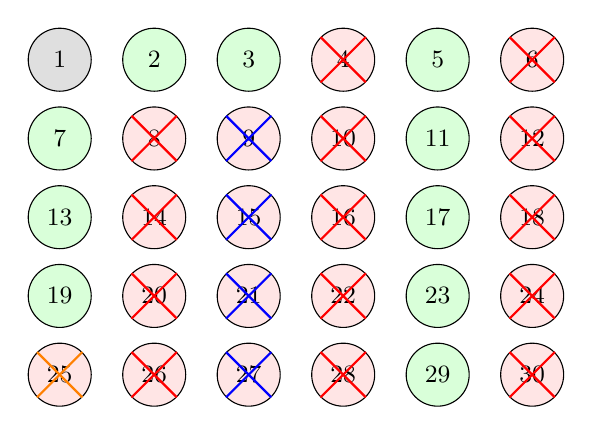
\begin{tikzpicture}[
  node/.style={circle, draw, minimum size=0.8cm, font=\small, inner sep=0pt},
  prime/.style={circle, draw, fill=green!15, minimum size=0.8cm, font=\boldmath\small, inner sep=0pt},
  composite/.style={circle, draw, fill=red!10, minimum size=0.8cm, font=\small, inner sep=0pt},
  neutral/.style={circle, draw, fill=gray!25, minimum size=0.8cm, font=\small, inner sep=0pt}
]
% Grid Layout for 1 to 30
% Row 0 (1 to 6)
\node[neutral] (n1) at (0,4) {1};
\node[prime] (n2) at (1.2,4) {2};
\node[prime] (n3) at (2.4,4) {3};
\node[composite] (n4) at (3.6,4) {4};
\node[prime] (n5) at (4.8,4) {5};
\node[composite] (n6) at (6.0,4) {6};

% Row 1 (7 to 12)
\node[prime] (n7) at (0,3) {7};
\node[composite] (n8) at (1.2,3) {8};
\node[composite] (n9) at (2.4,3) {9};
\node[composite] (n10) at (3.6,3) {10};
\node[prime] (n11) at (4.8,3) {11};
\node[composite] (n12) at (6.0,3) {12};

% Row 2 (13 to 18)
\node[prime] (n13) at (0,2) {13};
\node[composite] (n14) at (1.2,2) {14};
\node[composite] (n15) at (2.4,2) {15};
\node[composite] (n16) at (3.6,2) {16};
\node[prime] (n17) at (4.8,2) {17};
\node[composite] (n18) at (6.0,2) {18};

% Row 3 (19 to 24)
\node[prime] (n19) at (0,1) {19};
\node[composite] (n20) at (1.2,1) {20};
\node[composite] (n21) at (2.4,1) {21};
\node[composite] (n22) at (3.6,1) {22};
\node[prime] (n23) at (4.8,1) {23};
\node[composite] (n24) at (6.0,1) {24};

% Row 4 (25 to 30)
\node[composite] (n25) at (0,0) {25};
\node[composite] (n26) at (1.2,0) {26};
\node[composite] (n27) at (2.4,0) {27};
\node[composite] (n28) at (3.6,0) {28};
\node[prime] (n29) at (4.8,0) {29};
\node[composite] (n30) at (6.0,0) {30};

% Cross out composite numbers (X marks)
\foreach \i in {4,6,8,10,12,14,16,18,20,22,24,26,28,30} {
  \draw[red, thick] (n\i.south west) -- (n\i.north east);
  \draw[red, thick] (n\i.north west) -- (n\i.south east);
}
\foreach \i in {9,15,21,27} {
  \draw[blue, thick] (n\i.south west) -- (n\i.north east);
  \draw[blue, thick] (n\i.north west) -- (n\i.south east);
}
\foreach \i in {25} {
  \draw[orange, thick] (n\i.south west) -- (n\i.north east);
  \draw[orange, thick] (n\i.north west) -- (n\i.south east);
}
\end{tikzpicture}
\caption{Sieve of Eratosthenes execution up to $N=30$. Red lines indicate numbers eliminated by prime $2$, blue lines by prime $3$, and orange lines by prime $5$. Circled green numbers are the remaining primes.}
\label{fig:sieve}
\end{figure}

\section{Complexity Analysis and Proofs}
\label{sec:complexity}

\subsection{Time Complexity Proof}
We prove that the time complexity of the Sieve of Eratosthenes is $O(N \log \log N)$.

\begin{theorem}
The Sieve of Eratosthenes runs in $O(N \log \log N)$ operations.
\end{theorem}
\begin{proof}
For each prime $p \leq \sqrt{N}$, the algorithm marks its multiples. The number of multiples of $p$ less than or equal to $N$ is $\lfloor N/p \rfloor$. Summing this over all primes $p \leq N$:
\[
T(N) = \sum_{p \leq N} \frac{N}{p} = N \sum_{p \leq N} \frac{1}{p}
\]
By Mertens' Second Theorem, the sum of the reciprocals of prime numbers up to $N$ behaves asymptotically as:
\[
\sum_{p \leq N} \frac{1}{p} = \log \log N + M + o(1)
\]
where $M \approx 0.261497$ is the Meissel-Mertens constant.
Substituting this back into the summation:
\[
T(N) = N (\log \log N + M + o(1)) = O(N \log \log N)
\]
Thus, the time complexity is $O(N \log \log N)$.
\end{proof}

\subsection{Space Complexity}
The space complexity is $O(N)$ because the algorithm requires a boolean array of size $N + 1$ to keep track of the primality status of each number.

\subsection{Optimizations}
\begin{itemize}
    \item \textbf{Odd-Only Sieving:} Since all even numbers greater than $2$ are composite, we can store only odd numbers in the boolean array. This reduces the space complexity to $N/2$ bits and doubles the execution speed.
    \item \textbf{Segmented Sieve:} For very large $N$, the boolean array may not fit in the cache. The segmented sieve divides the range $[1, N]$ into smaller segments of size $O(\sqrt{N})$. Primes in each segment are calculated sequentially. This reduces cache misses and lowers the active memory requirement to $O(\sqrt{N})$ space.
\end{itemize}

\section{Java Reference Implementations}
\label{sec:code}

\subsection{Restaurant Combinatorics (Zomato Combos)}
The following Java program identifies the restaurant with the highest variety of meal combos:
\begin{verbatim}
public class Solution {
    public int findMaxComboRestaurant(int[][] A) {
        if (A == null || A.length == 0) return -1;
        
        long maxCombos = -1;
        int bestRestaurantIndex = -1;
        
        for (int i = 0; i < A.length; i++) {
            // Apply the product rule
            long currentCombos = (long) A[i][0] * A[i][1] * A[i][2];
            if (currentCombos > maxCombos) {
                maxCombos = currentCombos;
                bestRestaurantIndex = i;
            }
        }
        return bestRestaurantIndex;
    }
}
\end{verbatim}

\subsection{Sieve of Eratosthenes}
The following Java program implements the Sieve of Eratosthenes to generate all primes between $1$ and $N$:
\begin{verbatim}
import java.util.ArrayList;

public class Solution {
    public ArrayList<Integer> sieveOfEratosthenes(int n) {
        if (n < 2) return new ArrayList<>();

        boolean[] isPrime = new boolean[n + 1];
        for (int i = 2; i <= n; i++) {
            isPrime[i] = true;
        }

        // Optimization: outer loop runs up to sqrt(n)
        for (int p = 2; p * p <= n; p++) {
            if (isPrime[p]) {
                // Mark multiples starting from p*p
                for (int i = p * p; i <= n; i += p) {
                    isPrime[i] = false;
                }
            }
        }

        ArrayList<Integer> primes = new ArrayList<>();
        for (int i = 2; i <= n; i++) {
            if (isPrime[i]) {
                primes.add(i);
            }
        }
        return primes;
    }
}
\end{verbatim}

\section{Conclusion}
\label{sec:conclusion}

This paper analyzed the mathematical and algorithmic foundations of combinatorics and prime number generation. We examined the product and sum rules of counting, illustrating their direct applications in restaurant combo selections and multi-route network paths. We formalized permutations and selections, proving the algebraic relations behind Pascal's identity. 

Additionally, we investigated primality generation using the Sieve of Eratosthenes, visualizing the sieving steps for $N=30$ with a structured TikZ layout. Through the application of Mertens' theorem, we provided a rigorous proof of the $O(N \log \log N)$ asymptotic time complexity bound. The Java reference models confirm the practicality of these counting and primality algorithms for modern data structures and systems engineering.

\begin{thebibliography}{9}
\bibitem{cormen} T.~H.~Cormen, C.~E.~Leiserson, R.~L.~Rivest, and C.~Stein, \emph{Introduction to Algorithms}, 4th~ed. MIT Press, 2022.
\bibitem{knuth} D.~E.~Knuth, \emph{The Art of Computer Programming, Volume 1: Fundamental Algorithms}, 3rd~ed. Addison-Wesley, 1997.
\bibitem{rosen} K.~H.~Rosen, \emph{Discrete Mathematics and Its Applications}, 8th~ed. McGraw-Hill, 2018.
\bibitem{hardy} G.~H.~Hardy and E.~M.~Wright, \emph{An Introduction to the Theory of Numbers}, 6th~ed. Oxford University Press, 2008.
\end{thebibliography}


\end{document}
